\hypertarget{distance_8c}{
\section{Referencia del Archivo distance.c}
\label{distance_8c}\index{distance.c@{distance.c}}
}


\subsection{Descripci\'{o}n detallada}
En este archivo se definen las diferentes funciones para encontrar la distancia entre varios objetos. 

Definici\'{o}n en el archivo \hyperlink{distance_8c-source}{distance.c}.

{\tt \#include $<$stdlib.h$>$}\par
{\tt \#include $<$math.h$>$}\par
{\tt \#include $<$float.h$>$}\par
{\tt \#include \char`\"{}distance.h\char`\"{}}\par
{\tt \#include \char`\"{}point.h\char`\"{}}\par
{\tt \#include \char`\"{}line.h\char`\"{}}\par
{\tt \#include \char`\"{}polygon.h\char`\"{}}\par


Dependencia gr\'{a}fica adjunta para distance.c:\begin{figure}[H]
\begin{center}
\leavevmode
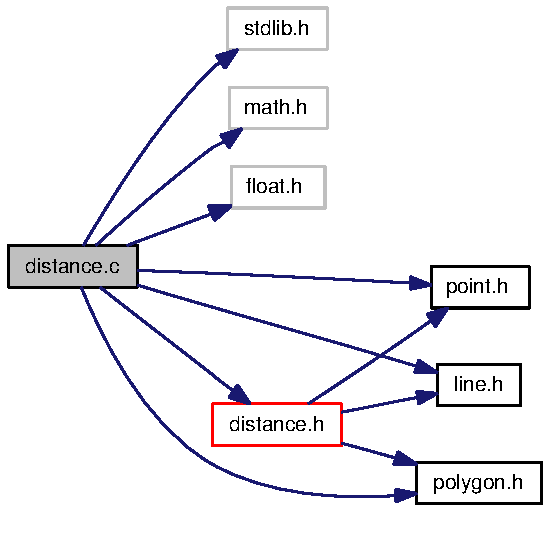
\includegraphics[width=150pt]{distance_8c__incl}
\end{center}
\end{figure}
\subsection*{Funciones}
\begin{CompactItemize}
\item 
float \hyperlink{group__distance_g3b2b03f846e6b587be683ec8b853e774_g3b2b03f846e6b587be683ec8b853e774}{distance\_\-pointpoint} (\hyperlink{struct__point}{point} $\ast$a, \hyperlink{struct__point}{point} $\ast$b)
\item 
float \hyperlink{group__distance_g69a59a49134b784b0c8797e0e83e7c40_g69a59a49134b784b0c8797e0e83e7c40}{distance\_\-pointline} (\hyperlink{struct__point}{point} $\ast$f, \hyperlink{struct__line}{line} $\ast$l, int $\ast$seg)
\item 
float \hyperlink{group__distance_g25716e8d1c8abaf08903bbcd08b8d6e5_g25716e8d1c8abaf08903bbcd08b8d6e5}{distance\_\-pointpolygon} (\hyperlink{struct__point}{point} $\ast$f, \hyperlink{struct__polygon}{polygon} $\ast$p, \hyperlink{struct__line}{line} $\ast$ref)
\item 
float \hyperlink{group__distance_gc837f0084791f42936ade857a0cce3af_gc837f0084791f42936ade857a0cce3af}{distance\_\-pointpolygonholes} (\hyperlink{struct__point}{point} $\ast$f, \hyperlink{struct__polygon__holes}{polygon\_\-holes} $\ast$p, \hyperlink{struct__line}{line} $\ast$ref)
\end{CompactItemize}
